\section*{Problem Statement}
The objective of this problem is to interpolate the position of the Earth around the Sun on a weekly basis, given the observed coordinates on the first week of each month. The goal is to use Lagrange interpolation to estimate the Earth’s position throughout the year and visualize the interpolated orbit.

\begin{quote}
  \textbf{NOTE}: The code can be accessed using this link: \href{https://raw.githubusercontent.com/HavokSahil/computational-techniques-assignments/refs/heads/main/assignment3/a2.m}{MATLAB}, \href{https://raw.githubusercontent.com/HavokSahil/computational-techniques-assignments/refs/heads/main/assignment3/a2.jl}{Julia}.
\end{quote}

\section*{Methodology}
The Earth’s orbit is approximately circular, but only monthly observations (12 data points) are available. To estimate weekly positions (48 weeks), an interpolating polynomial of degree $11$ was constructed separately for the $x$- and $y$-coordinates.

The Lagrange interpolation formula is:
\[
  P_k(x) = \sum_{i=0}^{k} f(x_i) \, L_i(x),
\]
where the basis polynomial $L_i(x)$ is defined as:
\[
  L_i(x) = \prod_{\substack{j=0 \\ j \neq i}}^{k} \frac{x - x_j}{x_i - x_j}.
\]

Here:
- $x_i$ corresponds to the week number of the observation,
- $f(x_i)$ corresponds to the observed coordinate ($X$ or $Y$).

Two independent interpolations were performed:
\[
P^{(x)}_{11}(\text{week}), \quad P^{(y)}_{11}(\text{week}),
\]
giving the parametric coordinates of Earth’s estimated orbit.

\subsection*{Pseudo-code}
\begin{enumerate}
  \item Store observed coordinates $(X, Y)$ for each month, along with corresponding week indices.
  \item Define Lagrange basis function $L_i(x)$.
  \item Define interpolating polynomial $P_k(x)$.
  \item For each week $w = 1, \dots, 48$:
    \begin{itemize}
      \item Compute interpolated $x = P^{(x)}_{11}(w)$.
      \item Compute interpolated $y = P^{(y)}_{11}(w)$.
    \end{itemize}
\end{enumerate}

\section*{Results}
The original monthly observations (12 points) are:
\[
(x,y) = \{(0.97,0.25), (0.80,0.60), (0.55,0.83), \ldots, (-0.31,-0.95)\}.
\]

Using degree-$11$ Lagrange interpolation, the Earth’s position was estimated for all 48 weeks. The figures show:
\begin{figure}[h!]
          \centering
          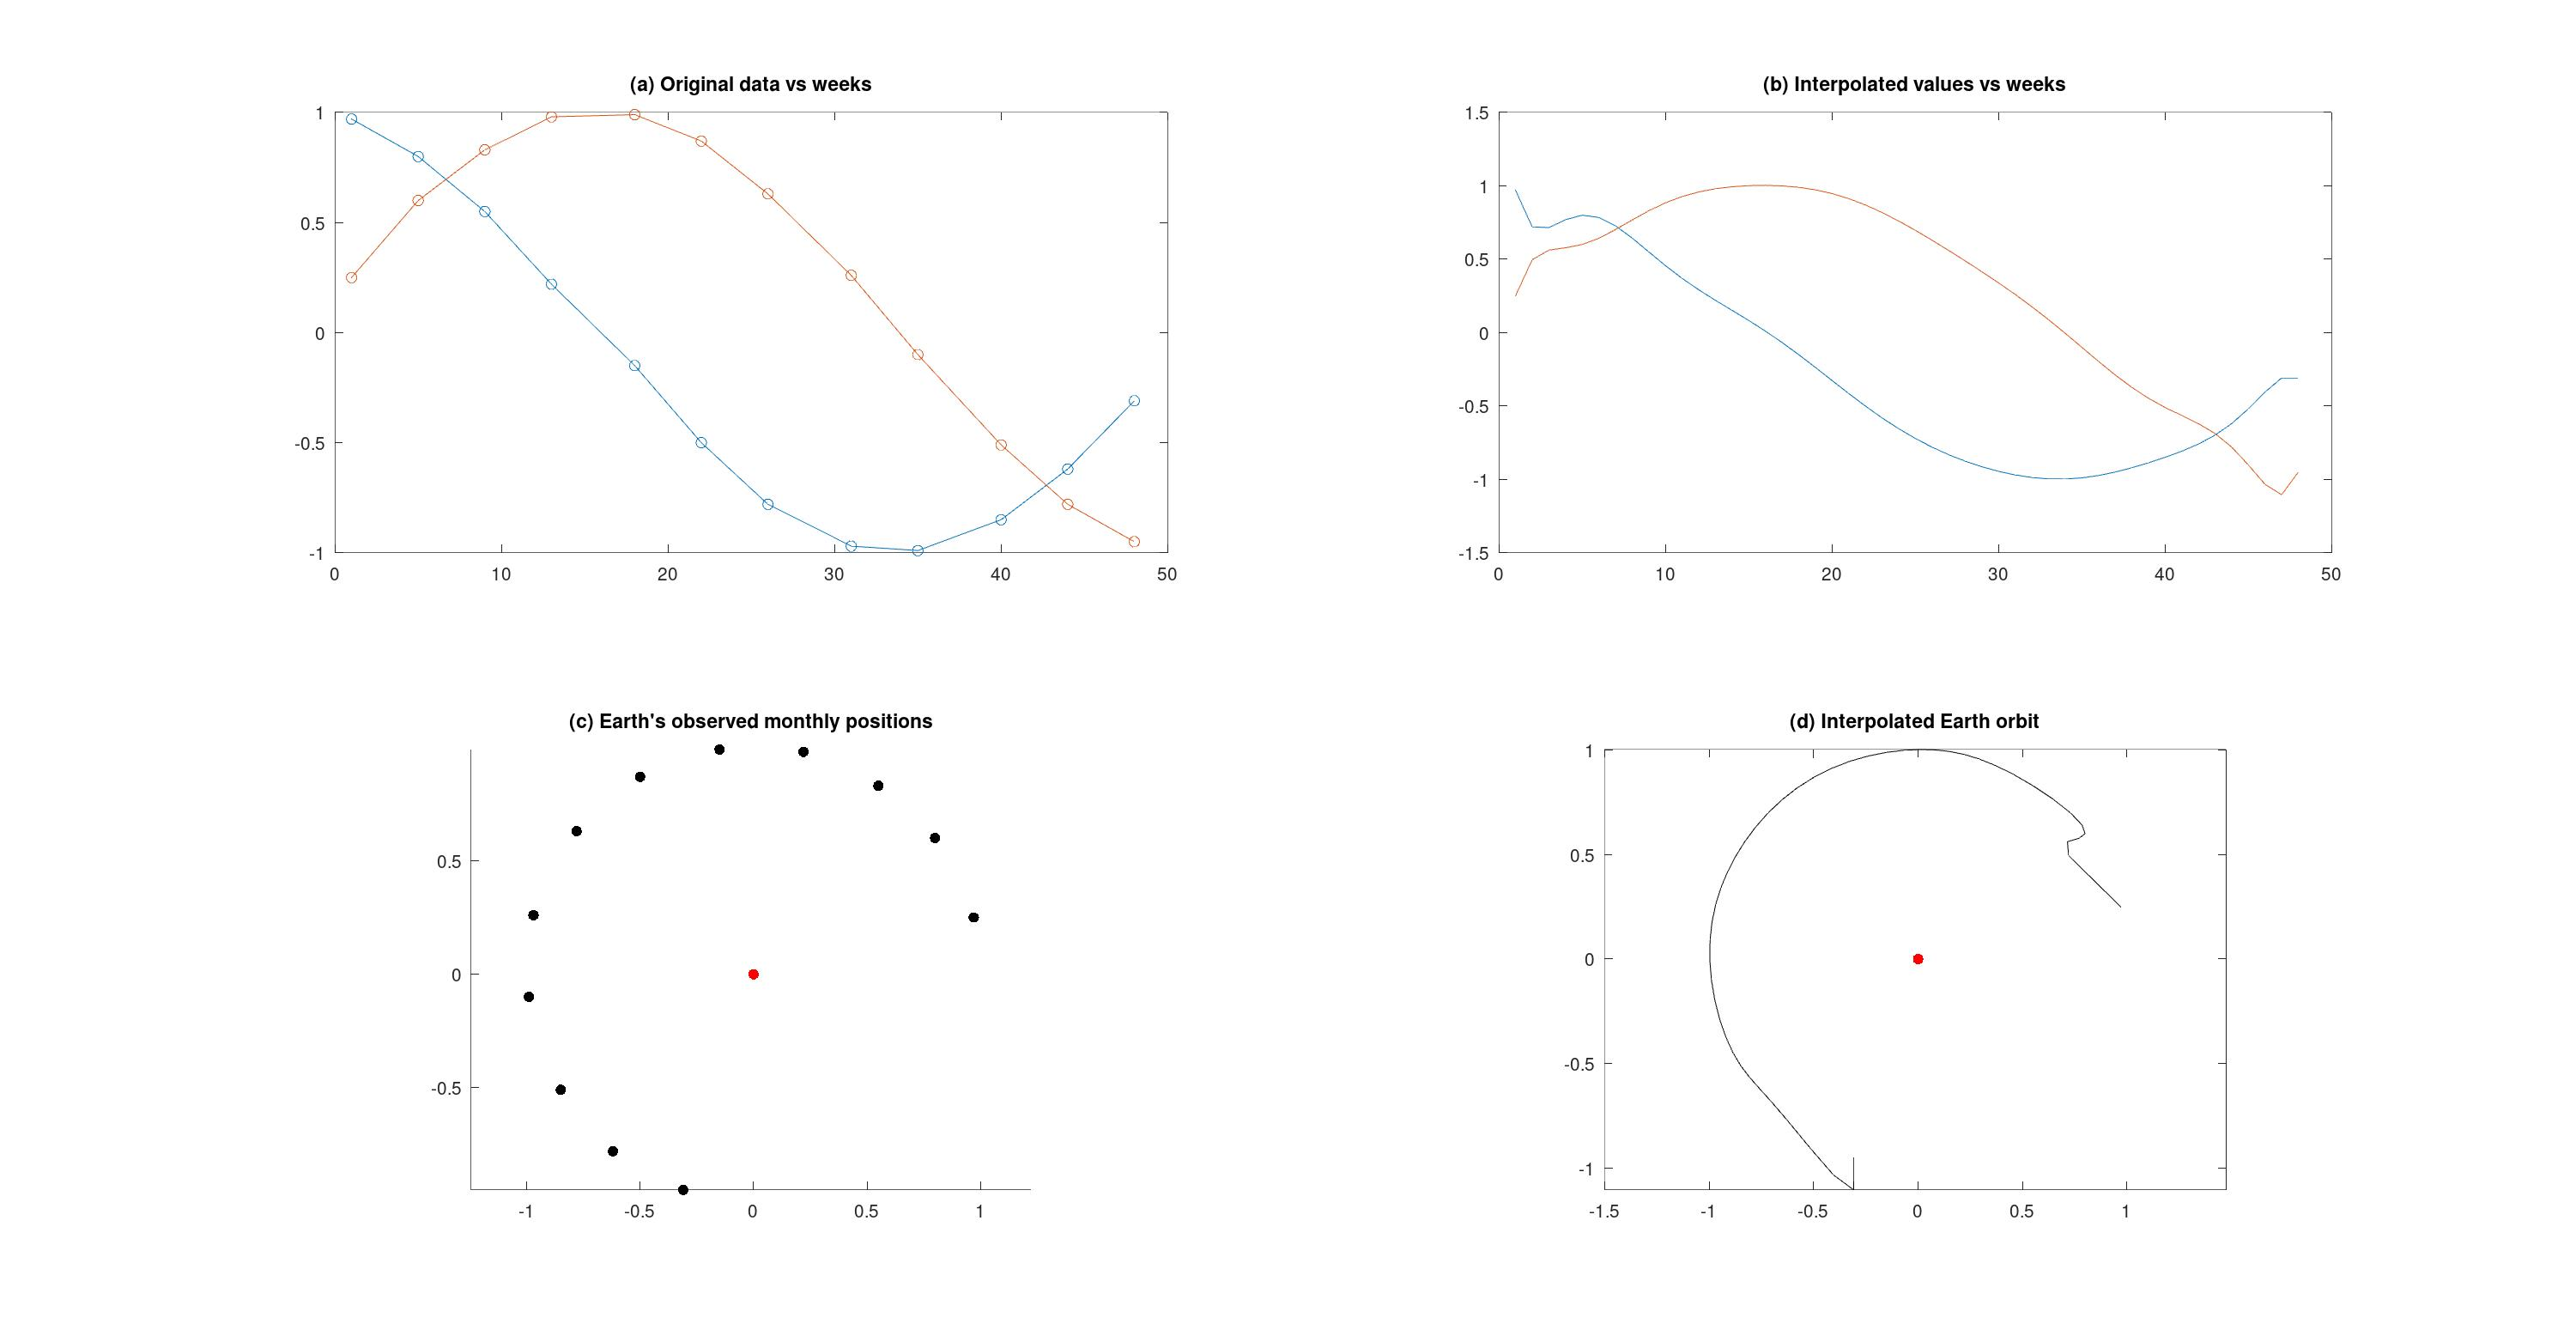
\includegraphics[width=1.0\textwidth]{a2.jpg}
          \caption{(a) Original monthly points forming a near-circular orbit. (b) Time evolution of $x$ and $y$ coordinates across 48 weeks. (c) Observed position data points around the sun (d) Interpolated orbit tracing a closed loop around the Sun.}
          \label{fig:a2}
\end{figure}

However, oscillations were observed at the edges of the interpolation domain (start and end weeks). As per my findings, this may be related to \textbf{Runge phenomenon}, where high-order polynomial interpolation over equally spaced points produces oscillations near the boundaries. \textit{However, any hints on this from the instructor would be invaluable.}

\section*{Conclusion}
The interpolated orbit successfully reconstructs the Earth’s approximate trajectory using only monthly data points. The Lagrange interpolation method provides a smooth approximation across weeks, but the observed edge oscillations highlight the limitations of high-order interpolation (Runge phenomenon).
